\documentclass{article}[18pt]
\usepackage{../../../../format}
\lhead{MODULE}
\usepackage{hyperref}
\usepackage{minted}[tabspace=4]

\providecommand{\tightlist}{%
	\setlength{\itemsep}{0pt}\setlength{\parskip}{0pt}}

\begin{document}
\begin{center}
\underline{\huge NODE JS}
\end{center}

\hypertarget{what-and-why}{%
	\section{What and Why?}\label{what-and-why}}

\begin{itemize}
	\tightlist
	\item
	Server-side scripting in JavaScript: alternative to php, asp, RoR
	\item
	Single thread execution: non-blocking
	\item
	Not designed for compute-heavy applications
	\item
	Package manager npm claims to be largest ecosystem of open source
	libraries in the world.
\end{itemize}

\begin{center}\rule{0.5\linewidth}{\linethickness}\end{center}

\hypertarget{history}{%
	\section{History}\label{history}}

\begin{itemize}
	\tightlist
	\item
	Developed from 2009
	\item
	Based on Chrome V8 Javascript engine: compiles to machine code
	\item
	Originally by Joyent, now has its own foundation
	\item
	\href{https://flaviocopes.com/node-history/}{Major fork in 2014} to
	io.js, since merged
	\item
	MIT-style licence
	\item
	Package manager npm (and yarn). See
	\href{https://blog.npmjs.org/post/141577284765/kik-left-pad-and-npm}{left
		pad incident}
\end{itemize}

\begin{center}\rule{0.5\linewidth}{\linethickness}\end{center}

\hypertarget{hosting}{%
	\section{Hosting}\label{hosting}}

\begin{itemize}
	\tightlist
	\item
	Cross-platform installation available for local hosting
	\item
	Available on many PaaS installations e.g.~openshift, IBM bluemix
	\item
	Not as widely available as php but more than most others (my
	opinion/experience)
\end{itemize}

\begin{center}\rule{0.5\linewidth}{\linethickness}\end{center}

\hypertarget{hello-world}{%
	\section{Hello world}\label{hello-world}}

\begin{minted}{js}
console.log("Hello world")
\end{minted}


\begin{itemize}
	\tightlist
	\item
	Save in hello.js
	\item
	run with \texttt{node\ hello.js}
	\item
	uses terminal as console instead of browser tools
\end{itemize}

\begin{center}\rule{0.5\linewidth}{\linethickness}\end{center}

\hypertarget{web-server}{%
	\section{Web server}\label{web-server}}

\begin{minted}{js}
http = require("http")

http.createServer(function (request, response) {
	response.writeHead(200, {'Content-Type': 'text/plain'});
	response.end('Hello World\n');
}).listen(8080);

console.log('Server running at http://127.0.0.1:8080/');
\end{minted}

\begin{center}\rule{0.5\linewidth}{\linethickness}\end{center}

\begin{itemize}
	\tightlist
	\item
	Use module http, based on CommonJS
	\item
	Module = file
	\item
	require returns a js object that contains the module components
	\item
	modules are installed with npm if necessary (plus dependencies)
	\item
	node starts its own web server rather than running as an apache module
	(like php often is)
\end{itemize}

\begin{center}\rule{0.5\linewidth}{\linethickness}\end{center}

\hypertarget{event-loop}{%
	\section{Event loop}\label{event-loop}}

\begin{itemize}
	\tightlist
	\item
	node runs on an event loop
	\item
	callbacks are associated with events
	\item
	programs should be non-blocking so that callbacks are provided for
	things like
	
	\begin{itemize}
		\tightlist
		\item
		block of data arrives from file
		\item
		block of data arrives from REST request
		\item
		results data arrives from database request
	\end{itemize}
	\item
	callbacks can themselves trigger new events
	\item
	next instruction is executed once all callbacks are complete
\end{itemize}

\begin{center}\rule{0.5\linewidth}{\linethickness}\end{center}


\begin{center}
	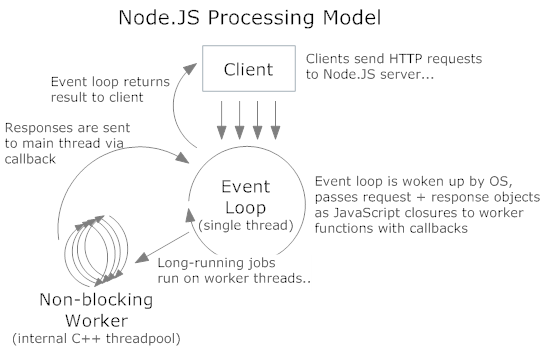
\includegraphics{image.png}
\end{center}





Thanks to
\href{http://stackoverflow.com/questions/14795145/how-the-single-threaded-non-blocking-io-model-works-in-node-js}{SO
	user568109}

\begin{center}\rule{0.5\linewidth}{\linethickness}\end{center}
\newpage
\hypertarget{hello-events}{%
	\section{Hello events}\label{hello-events}}

\begin{minted}{js}
var events = require('events');
var e = new events.EventEmitter();

function say(data){
	console.log("Hello " + data)
	e.emit('done')
}

e.on('say', say);

e.on('done', function(){
	console.log('Message done');
})

e.emit('say', 'world');

console.log('Program done');
\end{minted}

\begin{center}\rule{0.5\linewidth}{\linethickness}\end{center}

\hypertarget{routing-requests}{%
	\section{Routing requests}\label{routing-requests}}

\begin{itemize}
	\tightlist
	\item
	Variables can be GET-encoded
	\item
	In REST APIs they are often included in the URL directly (without
	question marks)
	\item
	E.g. use
	\href{https://developer.twitter.com/en/docs/api-reference-index}{twitter
		API}
	\item
	We want to use routing to pick bits out of the URL for this in nodejs
	\item
	There is a commonly used package called
	\href{http://expressjs.com/}{express}
\end{itemize}

\begin{center}\rule{0.5\linewidth}{\linethickness}\end{center}

\hypertarget{npm-packages}{%
	\section{npm packages}\label{npm-packages}}

\begin{itemize}
	\tightlist
	\item
	npm is your friend
	\item
	Dependencies are stored in package.json
	\item
	Uses \href{http://semver.org}{semantic versioning}
	
	\begin{itemize}
		\tightlist
		\item
		Code should have public API by version
		\item
		Version is X.Y.Z
		\item
		X = major version, Y = minor version, Z = patch
		\item
		Never change code within version once released
	\end{itemize}
\end{itemize}

\begin{center}\rule{0.5\linewidth}{\linethickness}\end{center}

\begin{itemize}
	\tightlist
	\item
	version semantics
	
	\begin{itemize}
		\tightlist
		\item
		X = 0 for pre-release versions
		\item
		Increase Z for bug-fixes, no new functionality
		\item
		Increase Y, set Z=0 for backwards-compatibile new functionality
		\item
		Increase X, set Y=Z=0 for backwards-incompatible new functionality
	\end{itemize}
	\item
	In package.json can use tilde to match minor version, caret to match
	major version etc
\end{itemize}

\begin{center}\rule{0.5\linewidth}{\linethickness}\end{center}
\newpage
\hypertarget{install-express}{%
	\section{Install express}\label{install-express}}

\begin{verbatim}
npm init
\end{verbatim}

creates package.json

\begin{verbatim}
npm install express
\end{verbatim}

installs express package and its dependencies

\begin{verbatim}
npm install express --save
\end{verbatim}

installs and puts dependency in package.json

\begin{center}\rule{0.5\linewidth}{\linethickness}\end{center}

\hypertarget{express-routing}{%
	\section{Express routing}\label{express-routing}}

\begin{minted}{js}
var express = require('express')
var app = express()

app.get('/', function(req, resp){
resp.send('Hello world')
})

app.listen(8090)
\end{minted}

This just starts an express app handling GET requests via port 8090

\begin{center}\rule{0.5\linewidth}{\linethickness}\end{center}

\begin{minted}{js}
var express = require('express')
var app = express()

app.get('/random/:max', function(req, resp){
max = parseInt(req.params.max)
rand = Math.floor(Math.random()*max) +1
console.log('Max via url is ' + max + ' rand is ' + rand)
resp.send('' + rand)
})

app.get('/r', function(req, resp){
max = parseInt(req.query.max)
rand = Math.floor(Math.random()*max) +1
console.log('Max via query is ' + max + ' rand is ' + rand)
resp.send('' + rand)
})

app.listen(8090)
\end{minted}

\begin{itemize}
	\tightlist
	\item
	Adds two separate routes
	\item
	Extract max value in two different ways
	\item
	Via value in URL (:max)
	\item
	Via value in GET-encoded variable
\end{itemize}

\begin{center}\rule{0.5\linewidth}{\linethickness}\end{center}


	\section{Popular tools for node}

\begin{itemize}
	\tightlist
	\item
	See list at \url{https://www.npmjs.com/}
	\item
	Killer app: \href{http://socket.io/get-started/chat/}{chat system}
\end{itemize}




\end{document}